\chapter{Параметри електрично активних \\ дефектів}\label{chapLevels}
Фізичні принципи значної частини методів дослідження дефектів
пов'язані зі зміною їхнього зарядового стану.
У зв'язку з цим розглянемо ці процеси детальніше.

Припустимо, що дефекту відповідає єдиний енергетичний рівень $E_t$,
розташований у забороненій зоні - див. рис.~\ref{F11}.
Залежно від того, зайнятий цей рівень чи ні (чи присутній в околі
порушення періодичності електрон з енергією $E_t$),
дефект може перебувати у двох зарядових станах.
Позначимо ці стани літерами А та В і припустимо,
що стану А відповідає випадок, коли в околі дефекту присутні $n_e$
електронів, а стану B --- на один електрон більше, ($n_e+1$).
В такій ситуації для позначення енергетичного рівня
нерідко використовують запис на кшталт $E_t(n_e/n_e+1)$,
причому початок відліку $n_e$ пов'язується з нейтральним станом
дефекту.
Так, наприклад, рівень легуючої донорної домішки
може бути записаний у вигляді $E_t(+1/0)$ або й навіть $E_t(+/0)$.
У дужках може наводитися і позначення лише одного зарядового стану,
який відповідає заповненому рівню ---  $E_t(n_e+1)$ для нашого модельного дефекту
і $E_t(0)$ для донора.

\begin{figure}[b]
\center
\vspace{-5mm}
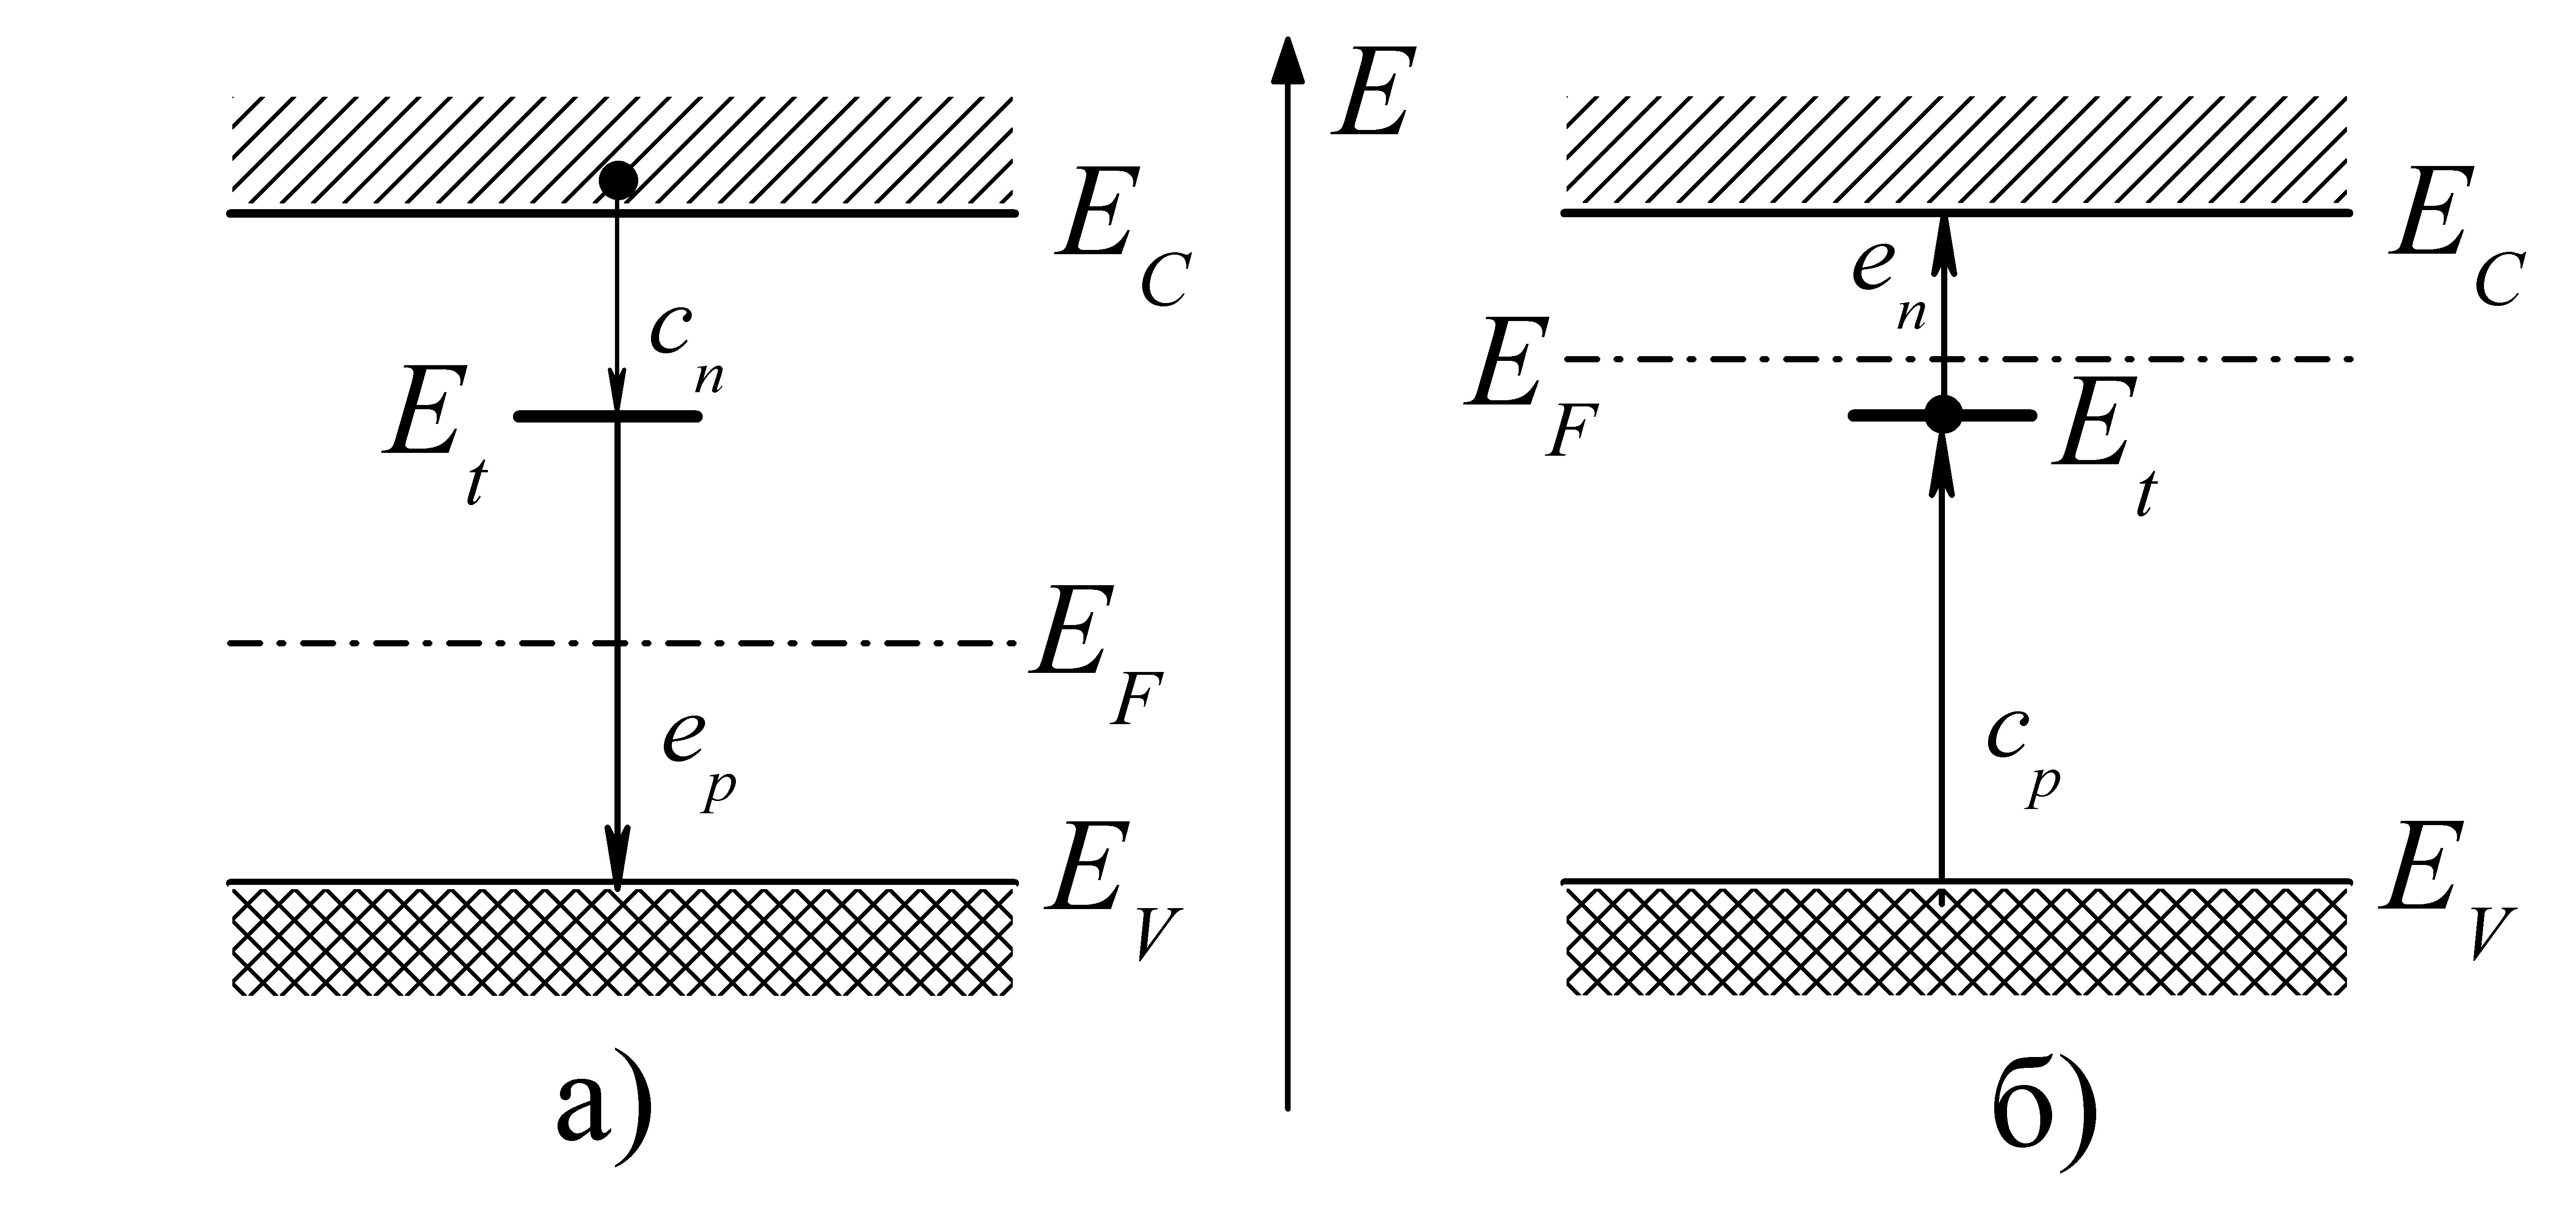
\includegraphics[width=0.8\textwidth]{Fig1_1}
\vspace{-3mm}
\caption{Схеми перезарядки дефектного рівня.}
\vspace{-3mm}
\label{F11}
\end{figure}

У випадку термодинамічної рівноваги співвідношення між концентраціями
дефектів у різних зарядових станах $N_{t,A}$ та $N_{t,B}$
наближено може бути записано у вигляді
\begin{equation}
\label{NbNa}
 \frac{N_{t,A}}{N_{t,B}}=\gamma_g\exp\left(-\frac{E_F-E_t}{kT}\right)\,,
\end{equation}
де $\gamma_g=g_{A}/g_{B}$,
 $g_{A}$ та $g_{B}$ --- кратності квантовомеханічного виродження станів А та В,
відповідно;
$E_F$ --- енергетичне положення рівня Фермі,
$k$ --- стала Больцмана,
$T$ --- температура.
Тобто, коли рівень Фермі знаходиться на енергетичній шкалі нижче рівня дефекту,
то останній переважно знаходиться у стані з меншою кількістю електронів (рис.~\ref{F11},а);
при зворотному співвідношенні між  $E_F$ та $E_t$  спостерігається ситуація,
коли $N_{t,B}>N_{t,A}$ (а частіше і $N_{t,B}\gg N_{t,A}$) --- рис.~\ref{F11},б.
Зауважимо, що на цьому рисунку незаповнений стан позначено горизонтальним штрихом,
а заповнений --- штрихом з кружечком.
Подібне позначення буде використовуватися і надалі.

Дефект може змінювати свій зарядовий стан, обмінюючись носіями заряду з дозволеними
зонами напівпровідника --- ці процеси показані на рис.~\ref{F11} стрілками.
Так, на рівень дефекту може переходити електрон з зони провідності;
кількість таких переходів за одиницю часу називається швидкістю (або темпом) захоплення електронів
і нерідко позначається $c_n$.
Процес переходу електрону з рівня дефекту у валентну зону (дірки з валентної зони)
описується за допомогою швидкості захоплення дірок $c_p$.
Перехід електрону з $E_t$ у зону провідності пов'язується зі швидкістю емісії електронів $e_n$.
Нарешті, швидкість емісії дірок $e_p$ характеризує процеси переходу
електрона з валентної зони на рівень дефекту (дірки з рівня дефекту у валентну зону).

Для темпів захоплення електронів із зони провідності та дірок з валентної зони
справедливі наступні співвідношення:
\begin{equation}
\label{cnp}
 c_n=n\,\sigma_n\,\upsilon_{th,n}\,, \qquad c_p=p\,\sigma_p\,\upsilon_{th,p}\,,
\end{equation}
де
$n$ та $p$ --- концентрації вільних електронів та дірок, відповідно,
$\sigma_n$ та $\sigma_p$ --- поперечні перерізи захоплення електронів та дірок
дефектом;
$\upsilon_{th,n(p)}$ --- теплова швидкість електронів (дірок):
\begin{equation}
\label{Vth}
 \upsilon_{th,n(p)}=\sqrt{\frac{3kT}{m_{n(p)}^*}}\,,
\end{equation}
$m_{n(p)}^*$ --- ефективна маса відповідного носія.

Поперечні перерізи захоплення носіїв є характеристиками
дефекту і залежать від його зарядового стану.
Зазвичай кулонівські притягуючі центри мають значно більший переріз ніж нейтральні,
які, в свою чергу, суттєво переважають за цим параметром відштовхуючі.
Згідно з емпіричним правилом, для притягуючих центрів  поперечний переріз захоплення
не менший ніж $10^{-14}$~см$^2$,
для нейтральних знаходиться в діапазоні $10^{-15}\div10^{-17}$~см$^2$,
а для відштовхуючих --- не більше $10^{-19}$~см$^2$.
Величини поперечних перерізів не залишаються постійними за будь-яких обставин.
Зокрема вони можуть залежати від температури, причому
характер температурної залежності визначається механізмом захоплення,
тобто тим, куди витрачається енергія, вивільнена при переході електрона на нижчий енергетичний рівень
(із зони провідності на рівень у забороненій зоні чи з $E_t$ у валентну зону).
Зокрема, згідно з \cite{ROUGIEUX2018},
якщо захоплення супроводжується процесом багатофонної емісії, то
переріз захоплення є термоактивованим:
\begin{equation}
\label{Sta}
 \sigma=\sigma_0\exp\left(-\frac{E_{\sigma}}{kT}\right)\,,
\end{equation}
де
$\sigma_0$ --- незалежна від температури константа;
$E_{\sigma}$ --- активаційна енергія;
при екситон--стимулюваному Оже--захопленні та каскадному захопленні
справедлива показникова залежність
\begin{equation}
\label{SAuger}
 \sigma=\sigma_0 T^{-\alpha_{\sigma}}\,;
\end{equation}
нарешті, для випадків класичного Оже--захоплення та радіаційного
захоплення (супроводжується випромінюванням фотону)
\begin{equation}
\label{Sklas}
 \sigma=\sigma_0\,.
\end{equation}
Величина показника ступеня в (\ref{SAuger}) може змінюватися у достатньо широких
межах, проте для електрично нейтрального центру нерідко $\alpha_{\sigma}=2$,
а для притягуючого (додатно зарядженого у випадку $\sigma_n$
та від'ємно зарядженого для $\sigma_p$) --- $\alpha_{\sigma}=1\div3$ \cite{Sachenko2017}.
Крім того, поперечний переріз захоплення може залежати від величини напруженості електричного поля \cite{Shishiyanu,Bourgoin2001}.


Повертаючись до процесів перезарядки, можемо записати
\begin{equation}
\label{dNdt}
 \frac{dN_{t,B}}{dt}=\left(c_n+e_p\right)N_{t,A}-\left(c_p+e_n\right)N_{t,B}\,.
\end{equation}
У стані термодинамічної рівноваги $dN_{t,B}/dt=0$.
Крім того, умова детальної рівноваги вимагає, щоб кількісно збігалися
процеси емісії та захоплення носіїв кожного типу.
%Якщо припустити, що загальна концентрація дефектів $N_t=dN_{t,B}+N_{t,A}$
%(тобто стани А та В є єдиноможливими для даного порушення періодичності),
%то для процесів, пов'язаних з електронами можемо записати
%\begin{equation}
%\label{rivn}
% c_n\left(N_{t}-N_{t,B}\right)=e_nN_{t,B}\,.
%\end{equation}
Так, для процесів, пов'язаних з електронами можемо записати
\begin{equation}
\label{rivn}
 c_nN_{t,A}=e_nN_{t,B}\,.
\end{equation}
Взявши до уваги рівності (\ref{NbNa}) та (\ref{cnp}), останній вираз набуває вигляду
\begin{equation}
\label{ecn}
e_n=c_n\gamma_g\exp\left(\frac{E_t-E_F}{kT}\right)=n\,\sigma_n\,\upsilon_{th,n}\gamma_g\exp\left(\frac{E_t-E_F}{kT}\right)\,.
\end{equation}
Відомо, що для невиродженого напівпровідника
\begin{equation}
\label{n}
n=N_C\exp\left(-\frac{E_C-E_F}{kT}\right)\,,
\end{equation}
де
$N_C$ --- густина енергетичних станів біля дна зони провідності,
$E_C$ --- енергія дна зони провідності.
А отже, темп емісії електронів має задовольняти наступному виразу
\begin{equation}
\label{en}
e_n=\sigma_n\,\upsilon_{th,n}\gamma_g N_C \exp\left(-\frac{E_C-E_t}{kT}\right)=\sigma_n\,\upsilon_{th,n}n_1\,,
\end{equation}
де
\begin{equation}
\label{n1}
n_1=\gamma_g N_C \exp\left(-\frac{E_C-E_t}{kT}\right)\,,
\end{equation}
дорівнює концентрації електронів у зоні провідності, коли рівень Фермі
співпадає з рівнем дефекту.
Цілком аналогічним чином можна отримати вираз для темпу емісії дірок:
\begin{equation}
\label{ep}
e_p=\sigma_p\,\upsilon_{th,p}p_1\,,
\end{equation}
де
\begin{equation}
\label{p1}
p_1=\gamma_p N_V \exp\left(-\frac{E_t-E_V}{kT}\right)\,,
\end{equation}
$N_V$ --- густина енергетичних станів біля стелі валентної зони,
$E_V$ --- енергія стелі валентної зони,
$\gamma_p=\gamma_g^{-1}=g_{B}/g_{A}$ (з точки зору цих носіїв заряду, стан В може інтерпретуватися як незаповнений діркою,
а стан А як заповнений).
Як видно з виразів (\ref{cnp}), (\ref{en}) та  (\ref{ep}),
швидкості захоплення носіїв заряду залежать від положення рівня Фермі,
тоді як швидкості емісії --- ні.

Якщо взяти до уваги, що
\begin{equation}
\label{Ncv}
N_C=\left(\frac{2\,\pi m_n^*\,k\,T}{h^2}\right)^{\frac{3}{2}}\,,\qquad N_V=\left(\frac{2\,\pi m_p^*\,k\,T}{h^2}\right)^{\frac{3}{2}}\,,
\end{equation}
та формулу (\ref{Vth}),
то температурну залежність швидкості емісії електронів можна записати у вигляді
\begin{equation}
\label{enT}
e_n=\beta\,\sigma_n(T)\,T^2 \exp\left(-\frac{E_C-E_t}{kT}\right)\,,
\end{equation}
де $\beta$ слабко залежить від температури.
Подібні співвідношення можна записати і для $e_p$, $c_p$ та $c_n$.

Зауважимо, що в стані термодинамічної рівноваги ймовірність заселеності рівня електроном $f_t$
визначається балансом захоплення та емісії носіїв заряду обох знаків:
\begin{equation}
\label{ft}
f_t=\frac{c_nn+e_p}{e_n+c_pp+c_nn+e_p}\,.
\end{equation}
За змістом це співвідношення близьке до (\ref{NbNa}).

До цього часу ми говорили про термічну емісію.
Проте процеси переходу носіїв у дозволені зони з локальних рівнів
у забороненій можуть ініціюватися і оптично.
В цьому випадку темп оптичної емісії електрону з глибокого рівня $e_n^o$
при опроміненні напівпровідника потоком фотонів $\Phi$ описується виразом
\begin{equation}
\label{enO}
e_n^o=\sigma_n^o\Phi\,,
\end{equation}
де
$\sigma_n^o$ --- оптичний переріз захоплення (або переріз фотоіонізації).
Ця величина залежить, зокрема, від частоти освітлення $\nu$ і в спрощеному випадку може
описуватися формулою Lucovsky \cite{tuomisto2019}
\begin{equation}
\label{SnO}
\sigma_n^o\sim \frac{1}{E_C-E_{t,o}} \left[\left(\frac{E_C-E_{t,o}}{h\nu}\right)\left(1-\frac{E_C-E_{t,o}}{h\nu}\right)\right]^{3/2}\,,
\end{equation}
де $(E_C-E_{t,o})$ --- оптична енергія іонізації дефекту.
В літературі запропоновані й більш точні моделі опису $\sigma_n^o$,
наприклад P\"{a}ssler \cite{Pasler_op} чи Vincent–-Chantre \cite{Chantre_op}.

Загалом, оптична енергія іонізації дефекту $E_C-E_{t,o}(n_e/n_e+1)$ може
відрізнятися від термічної енергії іонізації $E_C-E_{t}(n_e/n_e+1)$.
Конфігураційною діаграмою дефекту називається залежність його енергії
від узагальненої координати.
Останньою може бути зміщення атому, з яким пов'язаний дефект,
з точки високої симетрії, амплітуда релаксації атомів, що оточують дефект,
відстань між компонентами комплексного дефекту тощо.
Конфігураційна діаграма, як правило, характеризується наявністю основного мінімума,
розташування якого описує стабільну конфігурацію системи.
Проте далеко не завжди мінімум в різних зарядових станах спостерігається при
однаковому значенні узагальненої координати.

\begin{figure}[t]
\center
\vspace{-5mm}
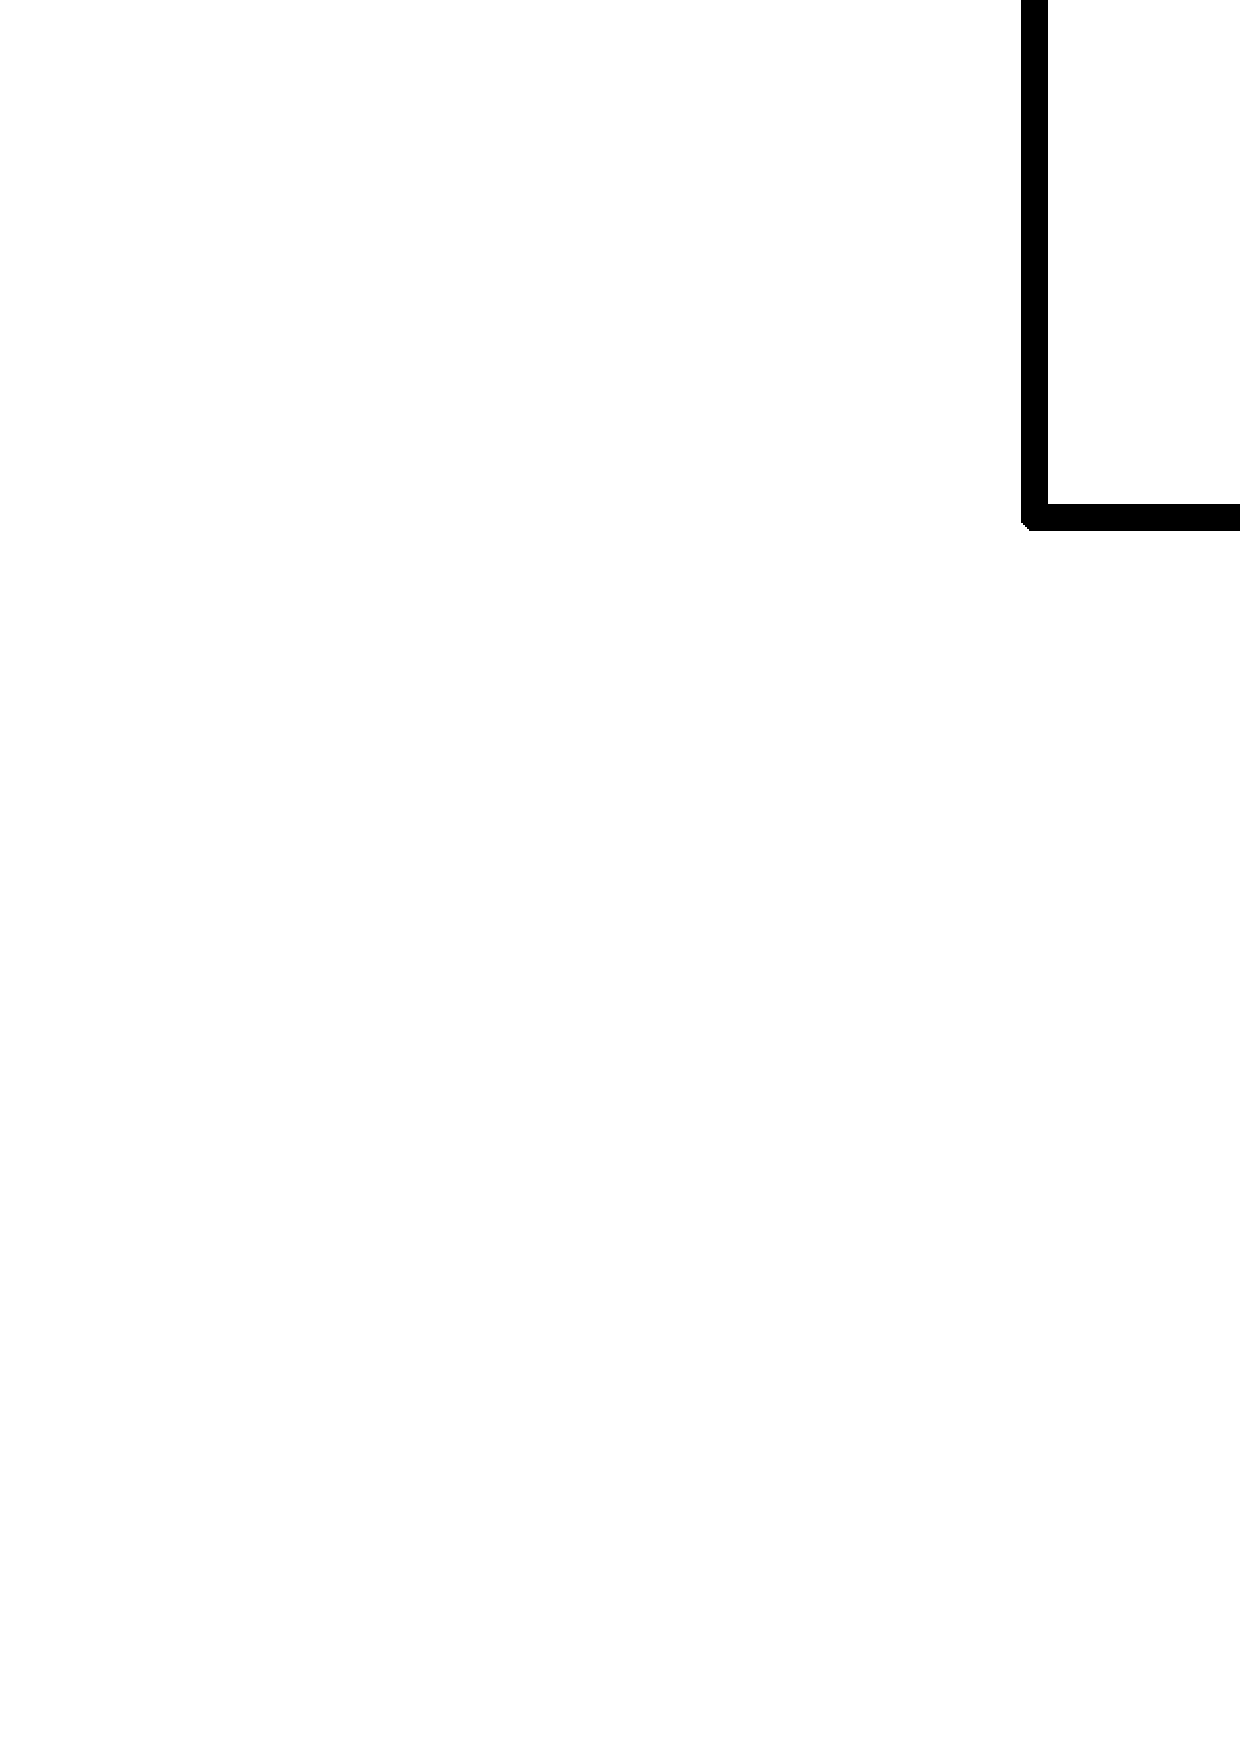
\includegraphics[width=0.7\textwidth]{Fig1_2}
\vspace{-3mm}
\caption{Схематична конфігураційна діаграма для пастки,
розташованій на відстані $E_C-E_{t}$ нижче дна зони провідності.
Нижня парабола відповідає енергії дефекту в стані В,
наступна --- енергії системи (дефект в стані А + вільний електрон),
верхня --- системи (дефект в стані В + вільний електрон + вільна дірка). %\\
Перехід 1 ілюструє оптичну емісію, 2 --- термічну.}
\vspace{-3mm}
\label{F12}
\end{figure}

Подібна ситуація зображена на рис.~\ref{F12},
де припускається, що станам дефекту А та В у рівновазі
відповідають різні узагальнені координати $Q_A^g$ та $Q_B^g\neq Q_A^g$.
Це означає, що при перезарядці дефекту для досягнення рівноваги
має змінитися просторове положення атомів.
Як правило, ці процеси значно повільніші, ніж електронний перехід
внаслідок поглинання фотона і тому під час фотоіонізації відбуватися не встигають.
Отже, оптично--стимульованій емісії на конфігураційній діаграмі відповідає вертикальний перехід
(1 на рис.~\ref{F12}).
В той же час, під час термічної емісії процес атомної релаксації  відбувається і тому
такий перехід на конфігураційній діаграмі має позначатися прямою, яка з'єднує мінімуми ---
перехід 2 на рис.~\ref{F12}.

Таким чином, оптичний рівень $E_{t,o}(n_e/n_e+1)$ асоціюється
з переходом між зарядовими станами (А та В), проте енергія кінцевого
стану має розраховуватися для атомної конфігурації початкового стану.
Оптичний рівень визначається, наприклад, у методах абсорбційної спектроскопії,
фотолюмінесценції, катодолюмінесценції, тобто коли у кінцевому
зарядовому стані не відбувається релаксація до рівноважної конфігурації.
Термічний рівень $E_{t}(n_e/n_e+1)$ може бути означений як положення рівня Фермі,
при якому стани А та В мають однакову енергію і при цьому у кінцевому після електронного переходу стані
мають повністю відбутися релаксаційні процеси.
Рівні такого типу спостерігаються в дослідженнях перехідної спектроскопії,
термостимульованих струмів, температуро-залежних холівських вимірах тощо.

Зауважимо, що на рис.~\ref{F12} також показані термоактиваційні енергії поперечних перерізів захоплення
заряду при багатофононному захопленні.
